\documentclass{beamer}
\usetheme{COURS}
\usepackage{tcolorbox}
\usepackage{textpos}
\usetikzlibrary{arrows,automata}
\usepackage{minted}
\usemintedstyle{emacs}


\def\red{\color{red}}
\def\blue{\color{blue}}
\def\green{\color{green}}

\def\opstyle#1{\ensuremath{\operatorname{#1}}}

\title[High Performance Combinatorics]%
{\bf High Performance Combinatorics}
\author{\textbf{\Large Florent Hivert}\\[5mm]
  Mél : \texttt{Florent.Hivert@lri.fr}\\
  Adresse universelle : \texttt{http://www.lri.fr/\~{ }hivert}
}
\date{}

\begin{document}
\newcommand{\Count}{\opstyle{count}}
\newcommand{\List}{\opstyle{list}}
\newcommand{\Iter}{\opstyle{iter}}
\newcommand{\Unrank}{\opstyle{unrank}}
\newcommand{\Rank}{\opstyle{rank}}
\newcommand{\First}{\opstyle{first}}
\newcommand{\Next}{\opstyle{next}}
\newcommand{\Random}{\opstyle{random}}

\newcommand{\Concat}{\opstyle{concat}}
\newcommand{\BS}{\opstyle{BitString}}
\newcommand{\Perm}{\opstyle{Perm}}
\newcommand{\Union}{\opstyle{Union}}
\newcommand{\Prod}{\opstyle{Prod}}

\newcommand{\Pos}{\opstyle{Pos}}
\newcommand{\Bin}{\opstyle{Bin}}
\newcommand{\Gray}{\opstyle{Gray}}

\newcommand{\mA}{\mathcal{A}}
\newcommand{\mB}{\mathcal{B}}
\newcommand{\mC}{\mathcal{C}}
\newcommand{\mD}{\mathcal{D}}
\newcommand{\mE}{\mathcal{E}}
\newcommand{\mI}{\mathcal{I}}
\newcommand{\mZ}{\mathcal{Z}}

\newcommand{\Oh}{O}

%***********************************************************************
\frame{\titlepage}
%***********************************************************************

\begin{frame}{Objectifs}
\Large

Montrer deux technologies qui permettent de rendre les calculs beaucoup plus
efficaces:\pause
\begin{itemize}
\item Instructions vectorielles entières pour les petits tableaux de nombres
\bigskip\pause

\item Parcours d'arbre récursif parallèle avec \texttt{Cilk++}
\end{itemize}
\end{frame}


\begin{frame}{Avertissement !!!}

Même si l'on obtient des gains très importants (x50, x500...), rien de tout
cela n'est de la \textbf{Bonne Informatique}\dots
\begin{itemize}
\item Technologie pas mure, bugs dans les compilateurs\dots
\bigskip\pause

\item Pas portable, y compris d'une version à l'autre du compilateur\dots
\bigskip\pause

\item Tentatives en cours de normaliser les syntaxes...
\end{itemize}
\end{frame}

\begin{frame}{Que retenir ?}

  \begin{NOTE}
    Les principes de parallélisation
    \begin{itemize}
    \item Vectorisation automatique ou manuelle
      \bigskip

    \item Parallélisation récursive
    \end{itemize}
  \end{NOTE}
  \bigskip\bigskip

  La syntaxe n'est \textbf{PAS} stable.
\end{frame}

\begin{frame}{Instruction vectorielles entières}

  Registre: \texttt{epi8,epu8}: 128~bits $=$ 16~octets
  \bigskip

  Encore plus: AVX, AVX2, AVX512
  \medskip

  \begin{itemize}
  \item Opérations Arithmetiques/logiques: \texttt{and, or, add, sub, min, max, abs, cmp}
  \item Recherche de bits: \texttt{popcount}, \texttt{bfsd}
  \end{itemize}
  \pause
  Encore plus intéressant pour nous:
  \begin{itemize}
  \item Manipulation de tableau: \texttt{blend, broadcast, shuffle}
  \item Comparaison de chaînes de caractères: \texttt{cmpistr} (lex, find).
  \end{itemize}
  \begin{tcolorbox}
    \centering
    \textbf{\large Manipulations très efficaces !}
  \end{tcolorbox}
\end{frame}

\begin{frame}{Exemple: les réseaux de tris}

  Knuth AoCP3 Fig.~51 p.~229:
  \[
  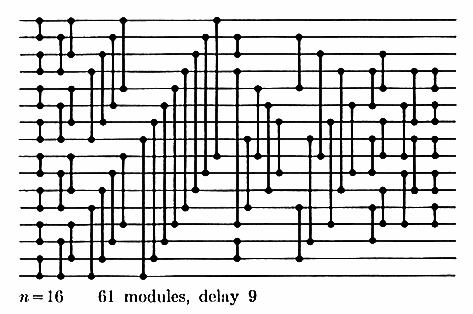
\includegraphics[height=5cm,width=11cm]{media/nibble-sort.png}
  \]
\end{frame}
\begin{frame}[fragile]

\small
\begin{minted}{C++}
// Sorting network Knuth AoCP3 Fig. 51 p 229.
static const array<perm, 9> rounds = {{
       { 1, 0, 3, 2, 5, 4, 7, 6, 9, 8,11,10,13,12,15,14},
       { 2, 3, 0, 1, 6, 7, 4, 5,10,11, 8, 9,14,15,12,13},
       ...
    }};
\end{minted}
\begin{minted}{C++}
perm sort(perm a) {
  for (perm round : rounds) {
    perm minab, maxab, mask;
    perm b = _mm_shuffle_epi8(a, round);
    mask = _mm_cmplt_epi8(round, permid);
    minab = _mm_min_epi8(a, b);
    maxab = _mm_max_epi8(a, b);
    a = _mm_blendv_epi8(minab, maxab, mask);
  }
  return a;
}
\end{minted}
\end{frame}


\begin{frame}[fragile]{Exemple 2: les cycles dans les permutations}

  $\left(\begin{array}{*{9}c}
      1&2&3&4&5&6&7&8&9\\
      1&6&9&7&8&2&4&3&5\\
    \end{array}\right)
  =(1)(2,6)(3,9,5,8,3)(4,7)$
  \bigskip

$O(n)$ algorithme utilisant $O(n)$ memoire.

\small
\begin{minted}{C++}
uint8_t nb_cycles_ref(Perm16 p) {
  Vect16 v {};
  int i, j, c = 0;
  for (i = 0; i < 16; i++) {
    if (v[i] == 0) {
      for (j=i; v[j] == 0; j = p[j]) v[j] = 1;
      c++;
    }
  }
  return c;
}
\end{minted}
\end{frame}


\begin{frame}[fragile]{Exemple 2: les cycles dans les permutations}

  $O(\log_2(n))$ algorithme utilisant $O(n)$ memoire.
  \medskip

  Idée: propager le minimum le long des cycles:
  \medskip

  {\def\s{\sigma}\def\m{\min}%
    \def\r#1{{\color{red}#1}}%
    \def\g#1{{\color{green}#1}}%
    \def\b#1{{\color{blue}#1}}%
  \small
  \[
  \begin{array}{l|*{16}c}
    i           & 0&\r{1}&2&\g{3}&4&5&\r{6}&7&\r{8}&\r{9}&a&b&\r{c}&d&\b{e}&\g{f} \\
    \s(i)       & d&\r{6}&b&\g{f}&5&2&\r{c}&4&\r{9}&\r{1}&7&0&\r{8}&a&\b{e}&\g{3} \\
    m:=\m(i,\s) & 0&\r{1}&2&\g{3}&4&2&\r{6}&4&\r{8}&\r{1}&7&0&\r{8}&a&\b{e}&\g{3} \\
    \hline
    \s^2(i)     & a&\r{c}&0&\g{3}&2&b&\r{8}&5&\r{1}&\r{6}&4&d&\r{9}&7&\b{e}&\g{f} \\
    s:=\s^2(\m) & 7&\r{8}&0&\g{3}&2&0&\r{8}&2&\r{1}&\r{6}&4&a&\r{1}&4&\b{e}&\g{3} \\
    m:=\m(m,s)  & 0&\r{1}&0&\g{3}&2&0&\r{6}&2&\r{1}&\r{1}&4&0&\r{1}&4&\b{e}&\g{3} \\
    \hline
    \s^4(i)     & 4&\r{9}&a&\g{3}&0&d&\r{1}&b&\r{c}&\r{8}&2&7&\r{6}&5&\b{e}&\g{f} \\
    s:=\s^4(\m) & 2&\r{1}&4&\g{3}&0&4&\r{1}&0&\r{1}&\r{1}&0&2&\r{6}&0&\b{e}&\g{3} \\
    m:=\m(m,s)  & 0&\r{1}&0&\g{3}&0&0&\r{1}&0&\r{1}&\r{1}&0&0&\r{1}&0&\b{e}&\g{3} \\
    \hline
    \s^8(i)     & 0&\r{8}&2&\g{3}&4&5&\r{9}&7&\r{6}&\r{c}&a&b&\r{1}&d&\b{e}&\g{f} \\
    s:=\s^8(\m) & 0&\r{1}&0&\g{3}&0&0&\r{1}&0&\r{1}&\r{1}&0&0&\r{1}&0&\b{e}&\g{3} \\
    m:=\m(m,s)  & 0&\r{1}&0&\g{3}&0&0&\r{1}&0&\r{1}&\r{1}&0&0&\r{1}&0&\b{e}&\g{3} \\
    \hline
    m == i      & 1&\r{1}&.&\g{1}&.&.&.&.&.&.&.&.&.&.&\b{1}&\g{.} \\
  \end{array}
  \]}
\end{frame}

\begin{frame}{Parallelisation avec \texttt{Cilk++}}
  

  \begin{NOTE}
    \begin{itemize}
    \item Programmation parallèle multifils en mémoire partagé.
      \bigskip\pause
    \item Extension du \texttt{C} et \texttt{C++}
      \bigskip\pause
    \item Ne pas écrire le parallélisme, mais l'exposer quand il est
      possible.
      \bigskip\pause
    \item Modèle Fork-Join:
\[\texttt{cilk\_spawn \qquad cilk\_sync}\]
    \end{itemize}
  \end{NOTE}
\end{frame}


\begin{frame}[fragile]{Fibonacci}
\begin{minted}{C++}
  int fib(int n) {
    if (n < 2) {
      return n;
    }
    else {
      int x, y;
      x = cilk_spawn fib(n - 1);
      y = cilk_spawn fib(n - 2);
      sync;
      return x + y;
    }
  }
\end{minted}
\end{frame}
\end{document}
